%!TEX root = ../main.tex
%
%
\begin{figure}[t]
\centering
\footnotesize
\begin{tabular}{@{}c@{\;}c@{\;}c@{\;}}
%Samples & Power spectrum & Radial mean \\
%
%=====================
%
%\rotatebox{90}{\qquad\quad multijitter} & 
\begin{tikzpicture}
  \node[anchor=south west,inner sep=0] (image) at (0,0)
  {
    \pdfliteral{ 1 w}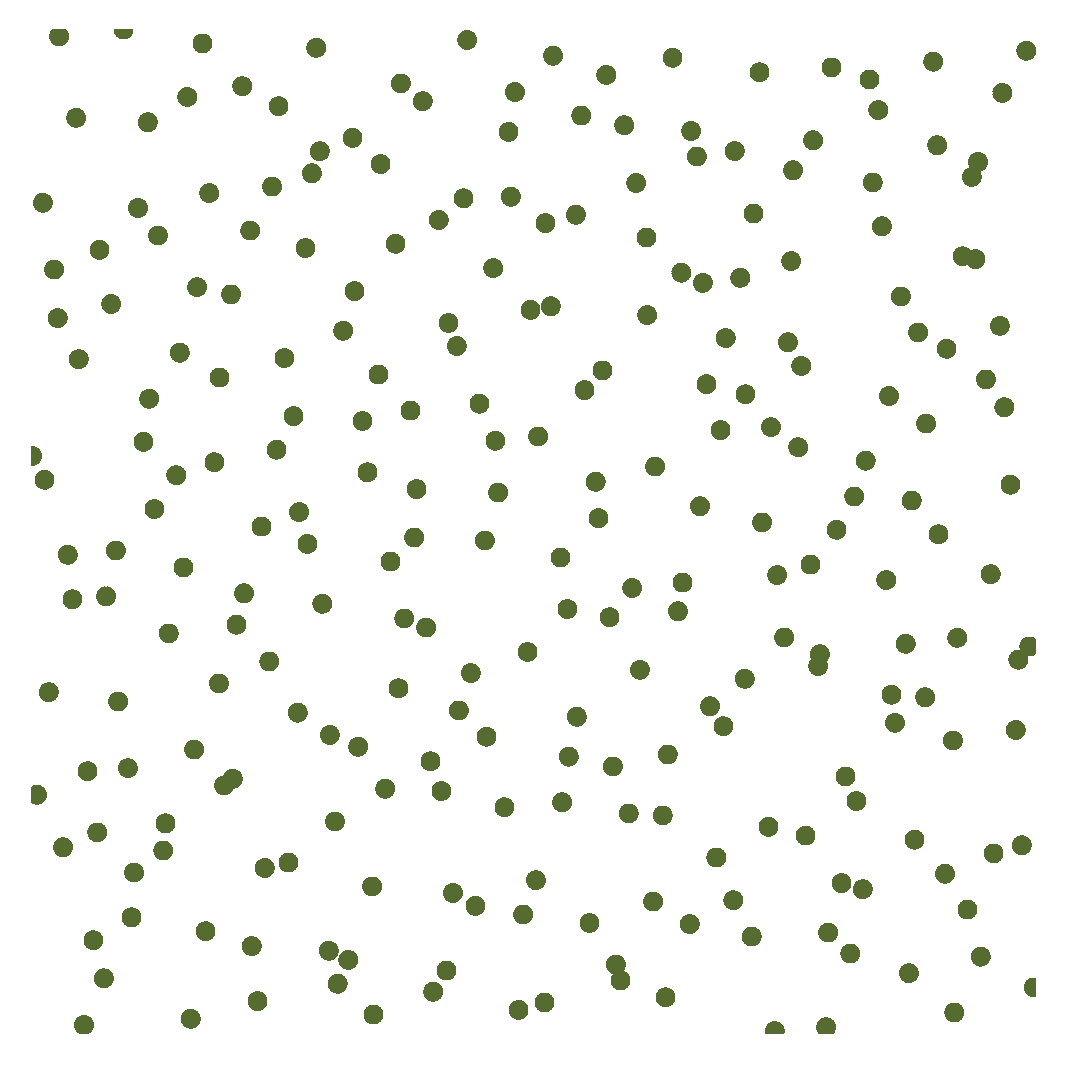
\includegraphics[width=1.4in,page=1]{pointset/points-multijitter-n256.pdf}
  };

  \begin{scope}[x={(image.south east)},y={(image.north west)}]
  \draw[black,thick] (0,0) rectangle (1,1);
  \end{scope}
\end{tikzpicture} 
&
\begin{tikzpicture}
  \node[anchor=south west,inner sep=0] (image) at (0,0)
  {
    \pdfliteral{ 1 w}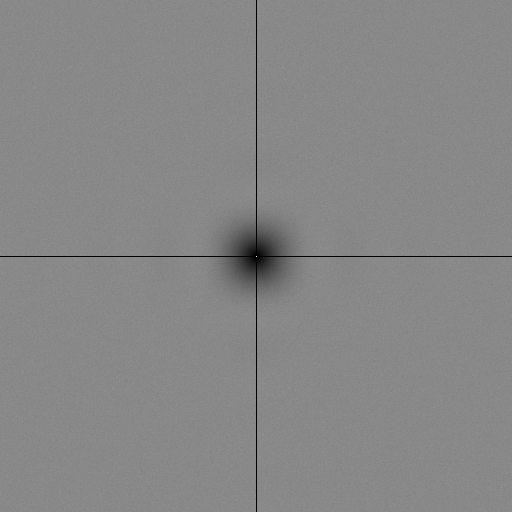
\includegraphics[width=1.4in,page=1]{power-spectra/powerspectrum-multijitter-n4096.png}
  };

  \begin{scope}[x={(image.south east)},y={(image.north west)}]
  \draw[black,thick] (0,0) rectangle (1,1);
  \end{scope}
\end{tikzpicture}
&
\begin{tikzpicture}
  \node[anchor=south west,inner sep=0] (image) at (0,0)
  {
    \pdfliteral{ 1 w}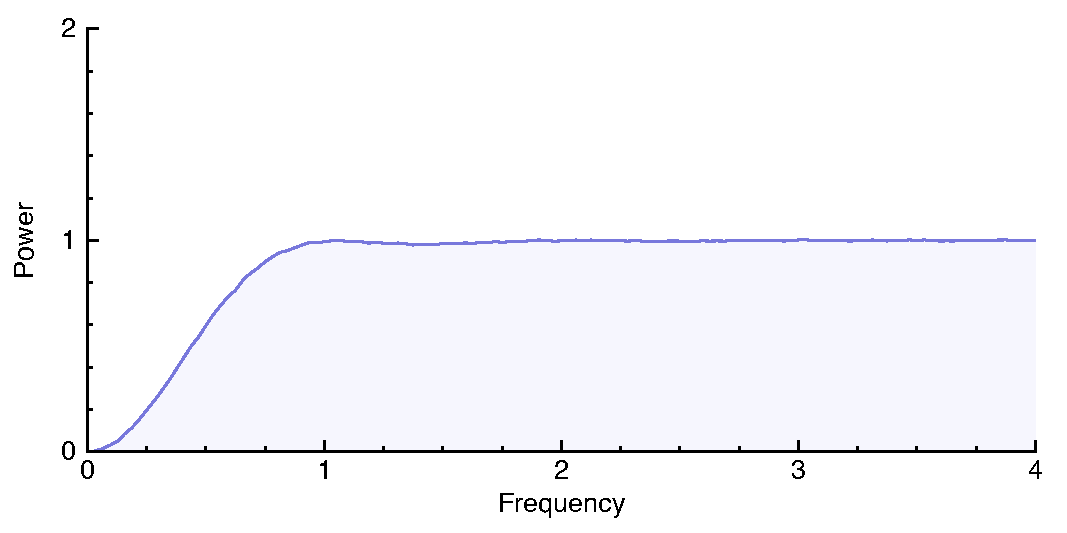
\includegraphics[width=2.8in,page=1]{power-spectra/radial-mean-multijitter-n1024.pdf}
  };

  \begin{scope}[x={(image.south east)},y={(image.north west)}]
  \draw[black,thick] (0,0) rectangle (1,1);
  \end{scope}
\end{tikzpicture}\\
\end{tabular}
\caption{\label{fig:powspec-radialmean-multijitter}%
Fourier analysis of multijittered samples.}
\end{figure}
%
